\section*{Chapter 10: Recurrent Neural Networks (RNNs)}
%\section*{Probabilities}
%\subsection*{Expect, Var, Cov, Bay}
%$\E[X]=\int_{\Omega}xf(x)\di x=\int_{\omega}x\Prob[X{=}x]\di x$ \\
Given an observation sequence $x^0, ..., x^s$, we want to identify hidden activities $h^t = F(h^{t-1}, x^t, \theta)$. $F$ can be a RNN $F(h, x; \theta) = \sigma(Wh + Ux + b)$. We can produce outputs $y = H(h; \theta) := \sigma(Vh + c)$.

Gradients vanish (or explode) for long sequences.

\textbf{Bi-directional RNN}. Take into account future by a reverse order sequence $g^t = G(x^t, g^{t+1}; \theta)$.

\textbf{Deep RNN}. Stack different hidden states and connect output to last hidden layer. $h^{t,1} = F^1(h^{t-1, 1}, x^t; \theta^1), ... h^{t,l} = F^l(h^{t-1, l}, h^{t, l-1}; \theta^l)$.

\subsection*{LSTM}
Their goal is to overcome the main limitation of RNNs: they forget quickly. Define gated units that can learn long-term dependencies.
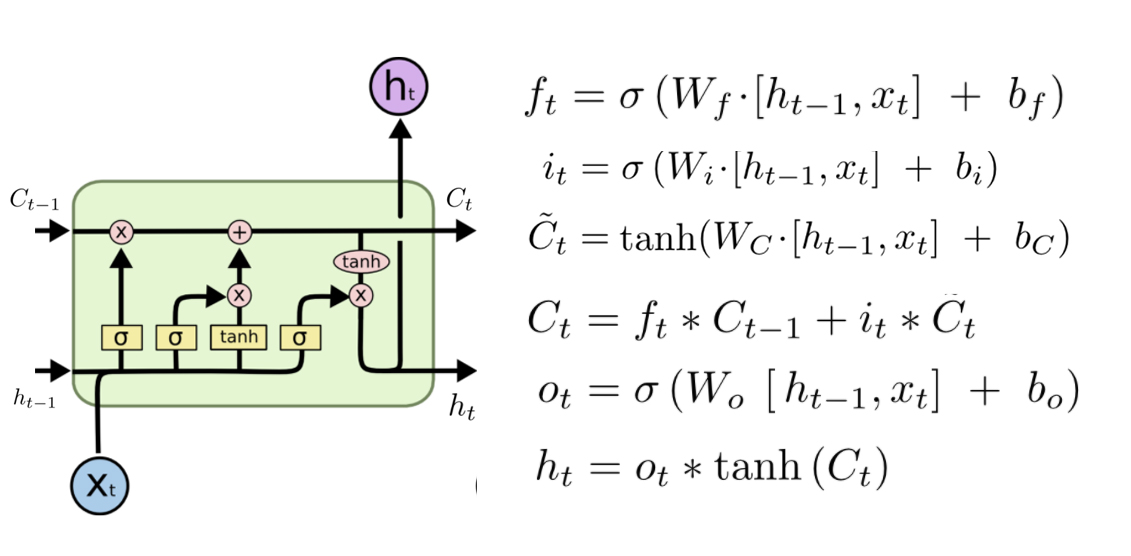
\includegraphics[width=\columnwidth]{src/lstm.jpg}
\subsection*{Gated memory units}
Simplified LSTM. Still difficult to train.
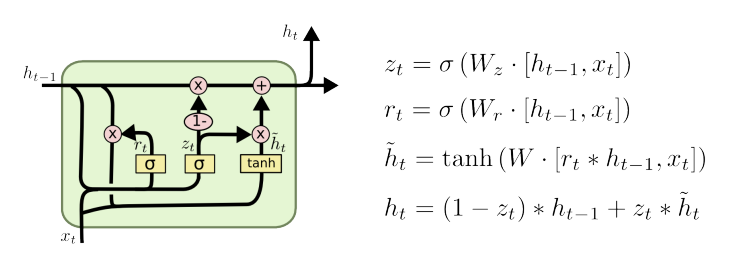
\includegraphics[width=\columnwidth]{src/gated-memory-units.png}

\subsection*{Learning sequences}
Goal: define cond. probability dist. over output sequence $y^{1:T}$ given inputs $x^{1:T}$ (special case: no input): $p(y^{1:T} | x^{1:T}) \approx \prod_{t=1}^Tp(y^t | x^{1:t}, y^{1:t-1})$.

A naïve RNN implementation would be: $x^{1:t} \xMapsto[]{F} h^t$; $h^t \xMapsto[]{H}\mu^t$; $\mu^t\xMapsto[]{H}p(y^t)$. The problem is that we assume $y^t$ is independent from $y^{t-1}$ (dependence through $h^t$). To overcome this, we can feedback previous outputs. 

\subsection*{Sequence-to-sequence learning}
Translate input sequence $x^{1:T}$ to $y^{1:T'}$. They might have diff. lengths and be unaligned. We build an encoder (RNN) that maps $x^{1:T} \mapsto z$ where $z=h^t$ (last hidden state). Then, a decoder maps $z \mapsto y^{1:T'}$. $z$ is "thought vector" that encodes the meaning of the sentence. It can be created from any model; e.g. a CV task.